\documentclass[tikz,border=3mm]{standalone}
\begin{document}
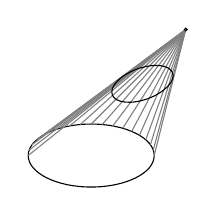
\begin{tikzpicture}[scale=.4]
\coordinate (A) at (0,0) {};
\draw (-3,-4) ellipse (2cm and 1cm);
\foreach \X in {0,10,...,180}
{
\draw[thin,gray] (A) -- ({-3+2*cos(\X)},{-4+sin(\X)});
}
\draw[fill=white] (A) circle (1.2pt);
\draw[rotate=20] (-1.88,-1.15) ellipse (1.02cm and .5cm);
\end{tikzpicture}
\end{document}
